

\begin{frame}{Portable Performance}

  \begin{block}{Scope for Portability Study}
    \begin{itemize}
     \item Vector and matrix-vector operations (BLAS levels 1 and 2)
     \item Limited by memory bandwidth
     %\item Matrix-matrix-multiplication (only briefly today)
    \end{itemize}
  \end{block}

  %\pause
  \begin{block}{Key Question (Memory-Bandwidth-Limited Kernels)}
    \begin{center} \color{red} \LARGE
     Good performance of complicated kernels \\
     by optimizing the simplest kernel?
    \end{center}
  \end{block}

\end{frame}


%% Copy kernel:
\begin{frame}[fragile]{Portable Performance}
  \begin{block}{Vector Assignment (Copy) Kernel}
    \begin{itemize}
     \item $x \Leftarrow y$ for (large) vectors $x$, $y$
    \end{itemize}
  \end{block}

  \only<1>{\vspace*{4.22cm}}
  \only<2>{\begin{center} \vspace*{0.84cm} 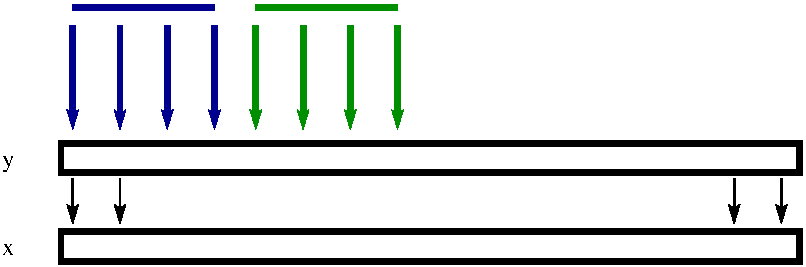
\includegraphics[width=0.8\textwidth]{figures/copy-kernel-gpu-1} \end{center}}
  \only<3>{\begin{center} \vspace*{0.85cm} 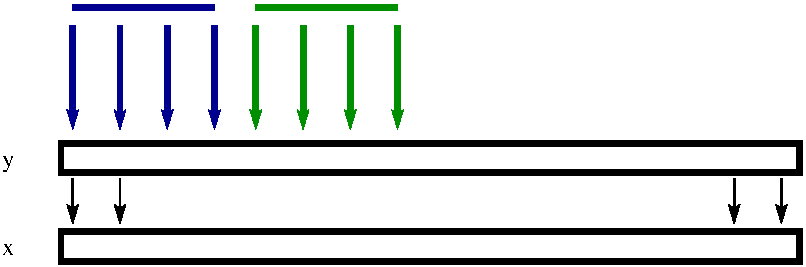
\includegraphics[width=0.8\textwidth]{figures/copy-kernel-gpu-1} \end{center}}
  \only<4>{\begin{center}                  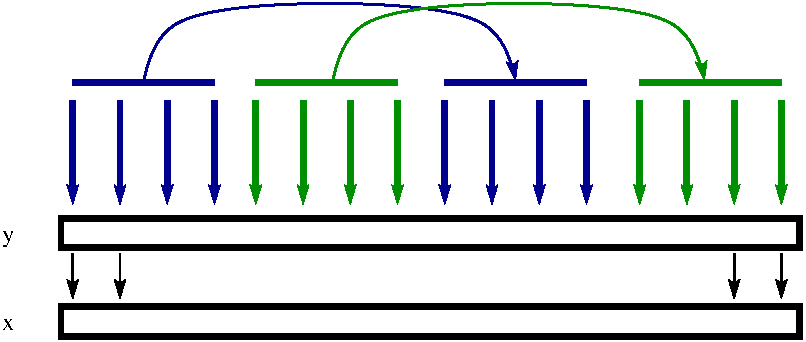
\includegraphics[width=0.8\textwidth]{figures/copy-kernel-gpu-full} \end{center}}
  \only<5>{\begin{center} \vspace*{0.84cm} 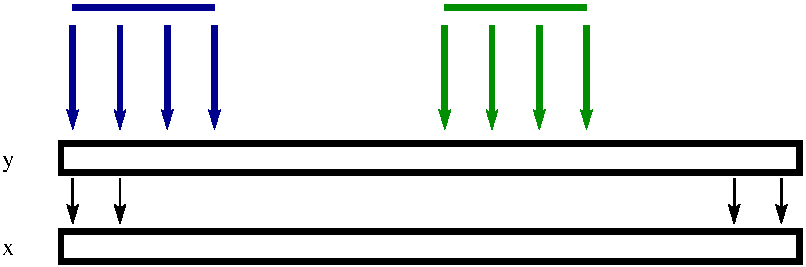
\includegraphics[width=0.8\textwidth]{figures/copy-kernel-cpu-1} \end{center}}
  \only<6>{\begin{center} \vspace*{0.30cm} 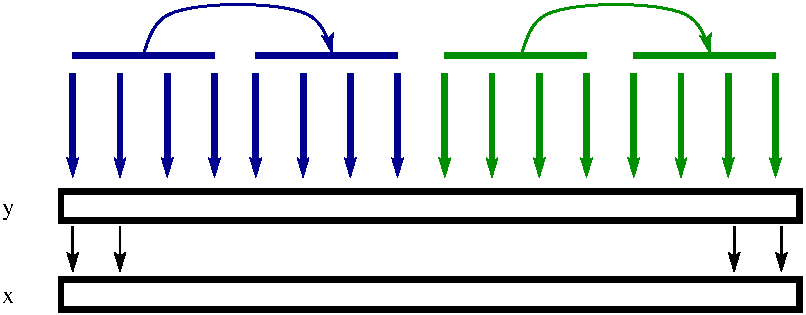
\includegraphics[width=0.8\textwidth]{figures/copy-kernel-cpu-full} \end{center}}
  
  \only<1>{\vspace*{2.52cm}}
  \only<2>{\vspace*{2.52cm}}
  \only<3>{
  \begin{block}{Parameters (1900 variations) }
   \begin{itemize}
    \item Local work size, global work size
    \item Vector types (float1, float2, ... , float16)
    \item Thread increment type
   \end{itemize}
  \end{block}}
  
  \only<4>{
  \begin{block}{Parameters (1900 variations) }
   \begin{itemize}
     \item \texttt{for (size\_t i = get\_global\_id(0); i < N;}
     \item \texttt{\ \ \ \ \ \ \ \ \ \ \ \ i+= get\_global\_size(0))}
     \item \texttt{\ \ x[i] = y[i];}
   \end{itemize}
  \end{block}
  }

  \only<5>{
  \begin{block}{Parameters (1900 variations) }
   \begin{itemize}
     \item \texttt{for (size\_t i = group\_start + get\_local\_id(0);}
     \item \texttt{\ \ \ \ \ \ \ \ \ \ \ \ i < group\_end;}
     \item \texttt{\ \ i+= get\_local\_size(0)) x[i] = y[i];}
   \end{itemize}
  \end{block}
  }

  \only<6>{
  \begin{block}{Parameters (1900 variations) }
   \begin{itemize}
     \item \texttt{for (size\_t i = group\_start + get\_local\_id(0);}
     \item \texttt{\ \ \ \ \ i < group\_end; i+= get\_local\_size(0)) }
     \item \texttt{\ \  x[i] = y[i];}
   \end{itemize}
  \end{block}
  }
\end{frame}


%% 
\begin{frame}{Portable Performance}

  \begin{block}{Operations}
   \begin{itemize}
    \item Vector copy, vector addition, inner product
    \item Matrix-vector product
   \end{itemize}
  \end{block}

  \only<1>{\begin{center} 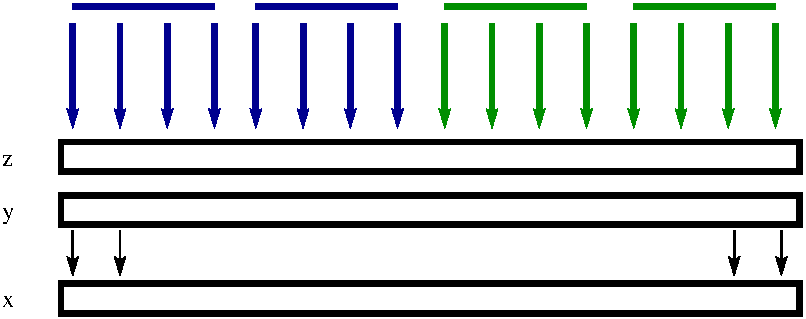
\includegraphics[width=0.8\textwidth]{figures/addition-kernel} \end{center}}
  \only<2>{\begin{center} 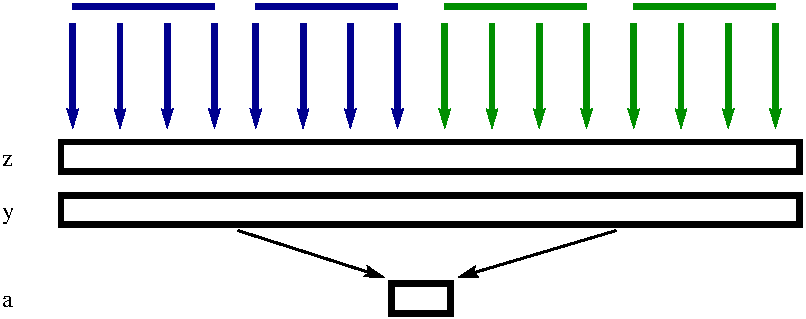
\includegraphics[width=0.8\textwidth]{figures/inner-product-kernel} \end{center}}
  \only<3>{\begin{center} 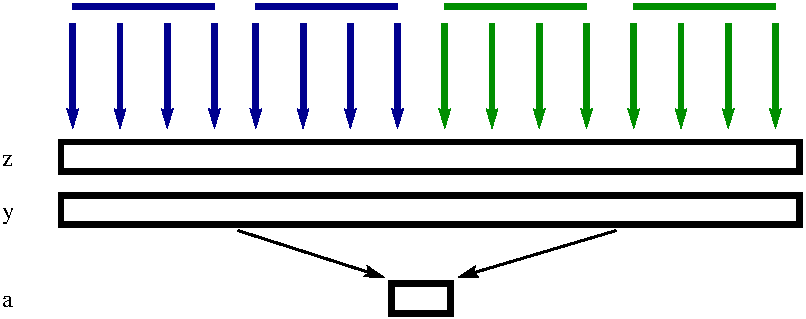
\includegraphics[width=0.8\textwidth]{figures/inner-product-kernel} \end{center}}

  \visible<3->{
  \begin{block}{Devices}
   \begin{itemize}
    \item AMD: Radeon HD 5850, FirePro W9000
    \item INTEL: Dual Socket Xeon E5-2670, Xeon Phi
    \item NVIDIA: GTX 285, Tesla K20m
   \end{itemize}
  \end{block}
  }
  
\end{frame}
